\chapter[2021 August]{August 2021}

\section[2021/08/08]{Sunday, 8 August 2021}

\subsection{STM32F103C8T6}

\subsubsection{Features}

The STM32F103C8T6 microcontroller has the following important features:

\begin{compactitem}
	\item 32-bit ARM Cortex M3 CPU Core with a maximum frequency of 72 MHz and single-cycle multiplication and division.
	\item 64 KB of flash (program) memory organised as 32-bit wide memory cells which may store both program data as well as the program code.
	\item 20KB of SRAM.
	\item 37 GPIOs.
	\item Word size of 32 bits and a half word size of 16 bits
\end{compactitem}

\subsubsection{Startup}

The selection of the system clock occurs when the system starts up. This is the internal 8 MHz oscillator by default. Alternatively, an external oscillator with a frequency in the range 4-16 MHz can be selected on startup. If this external oscillator fails, the RC oscillator will be selected instead by the system. On startup, the system may boot from User Flash, System Memory or the embedded SRAM which is selected using the boot pins. The SysTick timer is a timer that is dedicated for use by the \ac{OS} but may also be used as a downcounter.

\subsubsection{Programming}

The Flash memory embedded in the STM32F103C8T6 can be programmed using either \ac{ICP} or \ac{IAP}. \ac{ICP} involves updating the entirety of Flash memory with the application using the \ac{JTAG} protocol, \ac{SWD} protocol or the boot loader. On the other hand, \ac{IAP} allows the Flash memory to be reprogrammed while the application is running by means of any supported communication interface. The Cortex M3 core integrated two debug ports for both \ac{JTAG} as well as \ac{SWD}.

\pendsign

\section[2021/08/13]{Friday, 13 August 2021}

\subsection{Z-Axis Mount}

It was decided to use aluminium v-slot extrusions as the foundation of the robotic subsystem primarily due to the design flexibility offered this structure. The profile of the extrusion offers considerable stiffness required by the frame structure as well as mounting locations along any position of the structure by means of T-nuts. Furthermore, the v-shape present along the grooves in the extrusion allow the extrusion to be used as a linear guide. The extrusion was not considered as an option for a linear guide in the z-axis assembly due to its comparatively large mass compared to the mass of the z-assembly. However, in comparison to the mass of the x-axis assembly, the mass of the extrusion is much more reasonable and offers greater structural support in comparison to other linear guides such as linear chromed steel rods. The fact that the aluminium v-slot extrusion approach was selected for the rest of the robotic subsystem structure combined with the reasons discussed earlier was considered sufficient to select an aluminium extrusion as the x-axis linear guide. To assist in countering the torque generated about the x-axis by the z-axis assembly, it was decided to use a 2040 aluminium v-slot extrusion as opposed to a 2020 aluminium v-slot extrusion.

Linear motion along the aluminium v-slot extrusion is facilitated by v-slot wheels that run along the v-shaped grooves of the extrusion. Therefore, a need for a component to connect the z-axis assembly to the x-axis aluminium v-slot extrusion arose. The specific requirements of the required component are outlined below:

\begin{compactitem}
	\item The component needs to connect the 4 v-slot wheels positioned to run along the 2040 aluminium v-slot extrusion to the 4 linear bearings through which the linear chromed steel rods of the z-axis assembly run.
	\item The component needs to accommodate the excess movement required by the eccentric nuts used by half of the v-slot wheels.
	\item The component needs to provide mounting points for the timing belt on either side of the component.
	\item The component needs to provide a mounting point for the lead screw nut.
	\item The component needs to accommodate the length of the 8mm diameter to 5mm diameter rigid coupling used to attach the lead screw to the z-axis motor in the z-axis assembly. This accommodation allows the z-axis motor to move lower along the z-axis relative to the fixed linear bearings. This results in a shorter moment arm to the z-axis motor and reduces the torque about the x-axis.
	\item The component needs to be capable of being manufactured using \ac{FDM} 3D printing techniques.
	\item The component needs to support assembly with all of its supporting components.
\end{compactitem}

\begin{figure}[H]
	\centering
	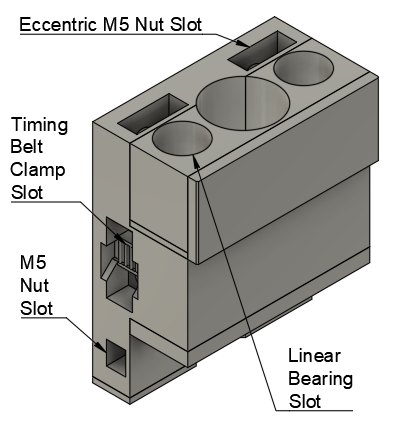
\includegraphics[width=0.35\linewidth]{figures/202108/z-axis-mount.png}
	\caption{Z-axis mount component for the z-axis assembly without supporting components.}
	\label{fig:z-axis-mount}
\end{figure}

\FigRef{fig:z-axis-mount} shows the z-axis mount developed to meet these requirements with various design features relating to these requirements highlighted. The walls of the eccentric spacer measure 1.76 mm and 0.34 mm. That means the bolt may be offset a maximum of 0.71 mm in any direction from the centre of the outer radius of the eccentric spacer which is accommodated in the design by the feature identified as the eccentric M5 nut slot.

The following components are used in conjunction with the z-axis mount:

\begin{compactitem}
	\item 4x delrin solid v-wheels
	\item 4x LM8UU linear bearings
	\item 8mm pitch delrin lead screw nut
	\item 2x eccentric nuts for v-wheels
	\item 4x M5x30 DIN 84 slotted cheese head machine screws
	\item 4x M5 washers
	\item 2x custom designed timing belt clamps
\end{compactitem}

\FigRef{fig:z-axis-mount-assembled} shows the z-axis mount assembled with all the components listed above is shown from an angled perspective from below the component. The 8mm pitch lead screw nut can be seen centred near the bottom of the component. One of the timing belt clamps can be seen placed over the timing belt clamp slot on the side of the z-axis mount.

\begin{figure}[H]
	\centering
	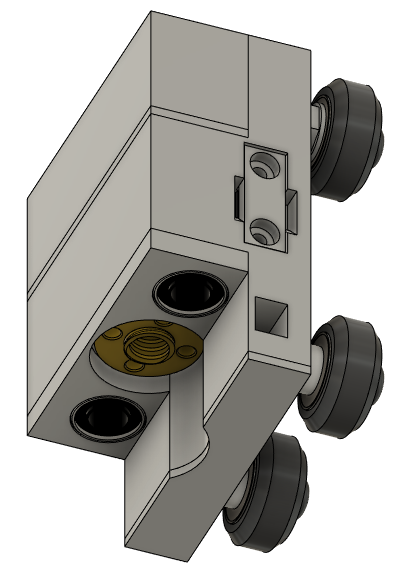
\includegraphics[width=0.3\linewidth]{figures/202108/z-axis-mount-assembled.png}
	\caption{Z-axis mount component for the z-axis assembly with supporting components.}
	\label{fig:z-axis-mount-assembled}
\end{figure}

\subsection{X-Axis Assembly}

For the purposes of this project, the x-axis assembly is defined in a similar manner to the z-axis assembly. Specifically, the x-axis assembly is the collection of components that move linearly along the x-axis when the x-axis drive motor is activated. Similar to the z-axis assembly, a decision needs to be made regarding whether to position the x-axis drive motor as part of the x-axis assembly or not. There is no significant benefit to including the x-axis motor as part of the x-axis assembly either than it potentially reduces the complexity of the x-axis mount which no longer needs to support the motor as well. However, this is offset by the complexity increase in the z-axis mount which would need to include a mounting point for the x-axis motor. Furthermore, mounting the motor in this manner would increase the mass of the x-axis assembly which would require a larger motor with more torque to drive. For these reasons, it was selected to not include the x-axis motor in the x-axis assembly. Note, the x-axis assembly does not include the x-axis linear guide in the form of the 2040 aluminium v-slot extrusion as it does not move when the x-axis drive is activated.

The second design consideration is the selection of the drive mechanism. Again, a lead screw approach was considered against a timing belt based approach. In this situation, the drive mechanism does not need to work directly against gravity as was the case with z-axis assembly. Furthermore, the range of motion of the x-axis assembly is significantly greater than that of the z-axis assembly. Based on these factors, in conjunction with the discussion of the drive mechanisms covered during the z-axis assembly analysis, the timing belt approach was selected. Due to the existence of the v-wheels to connect the z-axis mount to the aluminium extrusion, it was identified as being significantly more complicated to route the timing belt with the flat face parallel to the base plane. However, there were no obvious restrictions in routing the timing belt with the front face parallel to the x-axis aluminium v-slot extrusion. Furthermore, the aluminium v-slot extrusion facilitates the routing of the far side of the belt through the centre of the extrusion. For these reasons, it was decided to route the timing belt in this manner. Therefore, with all of the above considered, the x-axis assembly is defined to only consist of the z-axis mount as well as the z-axis assembly. \FigRef{fig:x-axis-assembly} shows x-axis assembly positioned on the x-axis aluminium v-slot extrusion.

\begin{figure}[H]
	\centering
	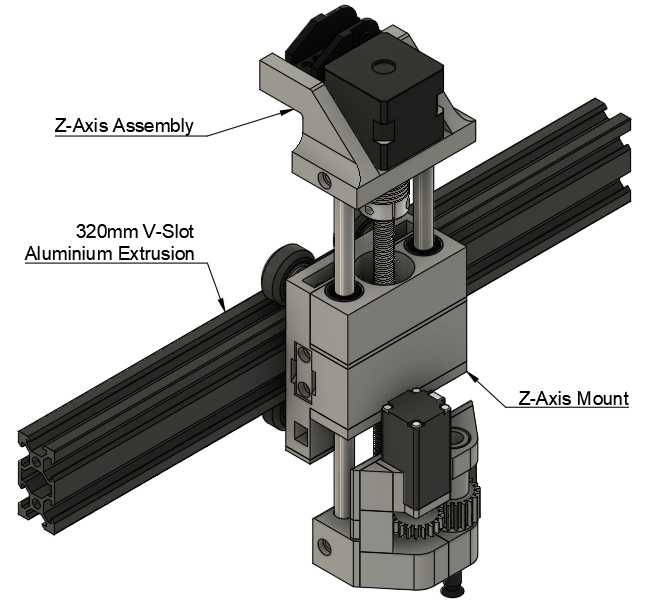
\includegraphics[width=0.8\linewidth]{figures/202108/x-axis-assembly.png}
	\caption{X-axis assembly consisting of the z-axis mount supporting the z-axis assembly.}
	\label{fig:x-axis-assembly}
\end{figure}

\subsection{Y-Axis Assembly}

For the purposes of this project, the y-axis assembly is defined in a similar manner to the z-axis and x-axis assemblies. Specifically, the y-axis assembly is the collection of components that moves linearly along the y-axis when the y-axis drive is activated. At this point in the design, the x-axis assembly is the highest level component of the robotic subsystem. The x-axis assembly runs along the x-axis aluminium v-slot extrusion. In order to introduce linear motion along the y-axis, both of these components need to be translated and therefore will both form part of the y-axis assembly.

In order to facilitate linear motion along the y-axis, linear guides need to be introduced into the design. Again, the most popular two linear guides were considered, namely the linear rail and the linear chromed steel rod. A consideration that applies to the y-axis motion that did not apply to the linear guides used on the other axes is the fact that the y-axis linear guides will always be fixed relative to the robotic structure. Therefore, weight is not a consideration in the selection of the linear guides. Furthermore, it has already been noted that aluminium v-slot extrusions are used to form the frame of the robotic subsystem. These extrusions facilitate simple mounting of linear rails by means of T-nuts. Furthermore, all of the mechanical advantages of the linear rail over the linear chromed steel rod as discussed earlier still apply. Since the y-axis assembly has the greatest mass of any of the moving components, the mechanical advantages offered by the linear rail were considered more relevant here than in earlier parts of the design. V-wheels were also considered as a means of linear motion along the v-slot aluminium extrusion. However, exploration of potential designs using this mechanisms exhibited many issues with routing the timing belt for the x-axis as well as the y-axis. Furthermore, the aluminium spacers would introduce additional length along the x-axis without any increase in the range of motion along the x-axis. 

For these reasons, the linear rail was selected as the linear guide along the y-axis. Furthermore, since both sides of the x-axis aluminium v-slot extrusion need to be supported, it was decided to use two linear rails, one on either side of the x-axis aluminium extrusion. The MGN12H linear bearing acts as the connection between the linear rail and the load item. Therefore, a requirement for two components to connect both ends of the x-axis aluminium extrusion to the MGN12H bearings arose. The requirements of the first component are as follows:

\begin{compactitem}
	\item The component needs to connect the left side of the x-axis 2040 aluminium v-slot extrusion to the left MGN12H linear bearing.
	\item The component needs to provide a mounting point for the 42BYGHW609 stepper motor such that the motor is in a position to drive the x-axis timing belt.
	\item The component needs to provide a timing belt clamping point on both sides of the component for the left y-axis timing belt.
	\item The component needs to facilitate the routing of the x-axis timing belt.
	\item The item needs to provide a mounting point for the end piece of the drag chain to facilitate the routing of wires and tubing originating from the z-axis assembly as well as the 42BYGHW609 stepper motor cables.
	\item The component needs to be capable of being manufactured using \ac{FDM} 3D printing techniques.
\end{compactitem}

\FigRef{fig:x-axis-mount-left} shows the left x-axis mount that was designed to meet these requirements along with indications of the roles of the various parts of the design. Similarly, the requirements of the second component are:

\begin{compactitem}
	\item The component needs to connect the right side of the x-axis 2040 aluminium v-slot extrusion to the right MGN12H linear bearing.
	\item The component needs to provide a mounting point for an idler pulley for a 6mm timing.
	\item The component needs to facilitate the movement of the idler pulley along the x-axis to allow the x-axis timing belt to be adjusted to the correct tension.
	\item The component needs to provide a timing belt clamping point on both sides of the component for the right y-axis timing belt.
	\item The component needs to facilitate the routing of the x-axis timing belt.
	\item The component needs to be capable of being manufactured using \ac{FDM} 3D printing techniques.
\end{compactitem}

\FigRef{fig:x-axis-mount-right} shows the right x-axis mount that was designed to meet these requirements along with indications of the roles of the various parts of the design.

\begin{figure}[H]
	\centering
	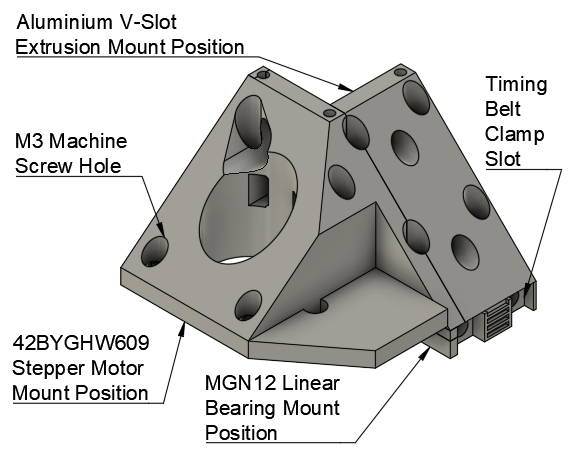
\includegraphics[width=0.45\linewidth]{figures/202108/x-axis-mount-left.png}
	\caption{X-axis assembly left mount.}
	\label{fig:x-axis-mount-left}
\end{figure}

\begin{figure}[H]
	\centering
	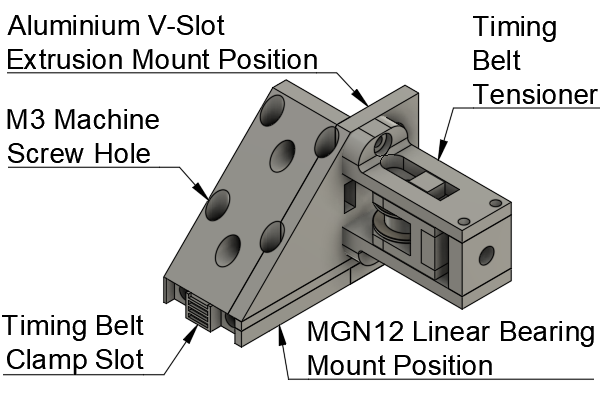
\includegraphics[width=0.4\linewidth]{figures/202108/x-axis-mount-right.png}
	\caption{X-axis assembly right mount.}
	\label{fig:x-axis-mount-right}
\end{figure}

The components that comprise the y-axis assembly are as follows:

\begin{compactitem}
	\item X-axis assembly
	\item X-axis 2040 aluminium v-slot extrusion of length 320mm
	\item Left x-axis mount
	\item Right x-axis mount
	\item 2x MGN12H linear bearings
	\item 42BYGHW609 stepper motor
	\item 4x custom timing belt clamps
	\item 20 tooth GT2 pulley for GT2 timing belt
	\item Idler pulley for 6mm belt
\end{compactitem}

\subsection{Final Assembly}

The highest level component of the robotic subsystem at this point in the design is the y-axis assembly. In order to complete the design, several components still need to be developed, namely the belt tensioners to be used on both the left and right y-axis timing belts as well as the y-axis drive mechanism. The y-axis belt tensioners have identical functions with the only difference being their operation on opposite sides of the robotic subsystem. Therefore, the left and right y-axis timing belt tensioners are mirror images of each other and essentially share the same design. The y-axis belt tensioner component needs to meet the following requirements.

\begin{compactitem}
	\item The component needs to provide a mounting point for the idler pulley for a 6mm timing belt.
	\item The component needs to facilitate mounting of itself to the aluminium v-slot frame of the robotic subsystem.
	\item The component needs to facilitate adjustment of the position of the idler pulley along the y-axis to allow the tension of the y-axis timing belt to be adjusted.
	\item The component needs to be capable of being manufactured using \ac{FDM} 3D printing techniques.
\end{compactitem}

\FigRef{fig:y-axis-belt-tensioner-right} shows the y-axis belt tensioner that was designed to fulfil these requirements on the right side of the robotic subsystem.

\begin{figure}[H]
	\centering
	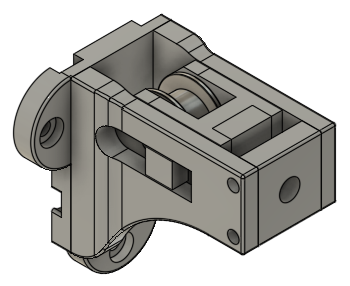
\includegraphics[width=0.4\linewidth]{figures/202108/y-axis-belt-tensioner-right.png}
	\caption{Y-axis belt tensioner for the right drive side.}
	\label{fig:y-axis-belt-tensioner-right}
\end{figure}

The second design that needs to be completed in order to complete the robotic subsystem is the y-axis drive mechanism. The primary requirement of this mechanism is that it needs to be capable of driving the y-axis timing belts on both the left and right side of the robotic subsystem. The obvious basis of this mechanism is to use a dual shaft stepper motor with each shaft used to drive one of the y-axis timing belts. The 42BYGHW920L21B2 stepper motor was selected for this characteristic. Unfortunately, the length of the stepper motor is not sufficient to drive each belt directly off each shaft. Instead it was decided to drive only the left side y-axis timing belt directly off the shaft using a 20 tooth pulley for a 6mm GT2 timing belt with a 5mm bore. In order to drive the right side y-axis timing belt, the torque needs to be transferred from the stepper motor shaft to a pulley connected to the timing belt. It was decided to use an 8mm linear chromed steel rod in order to transfer this torque to a 20 tooth pulley for a 6mm GT2 timing belt with a 8mm bore. An 8mm diameter to 5mm diameter coupling is required to connect the stepper motor shaft to the 8mm linear rod. The rigid coupling is not sufficient to support the linear rod along the drive axis. Therefore, two KP08 8mm pillow block bearings were introduced to support the linear rod. In order to connect the pillow blocks to the aluminium v-slot extrusion frame of the robotic subsystem, two custom connector components needed to be designed. Similarly, a component needed to be designed to connect the 42BYGHW920L21B2 stepper motor to the frame as well. All of the components discussed above form the y-axis drive mechanism which is shown attached to the robotic subsystem in \FigRef{fig:y-axis-drive-assembly}. The final robotic subsystem assembly is shown in \FigRef{fig:final-assembly}.

\begin{figure}[H]
	\centering
	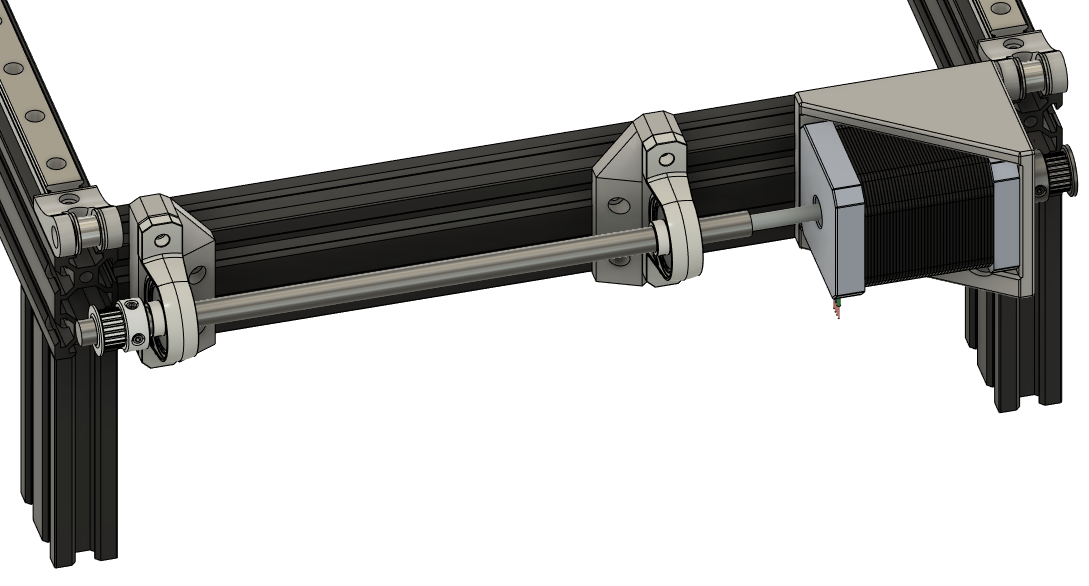
\includegraphics[width=0.7\linewidth]{figures/202108/y-axis-drive-assembly.png}
	\caption{Y-axis drive assembly.}
	\label{fig:y-axis-drive-assembly}
\end{figure}

\begin{figure}[H]
	\centering
	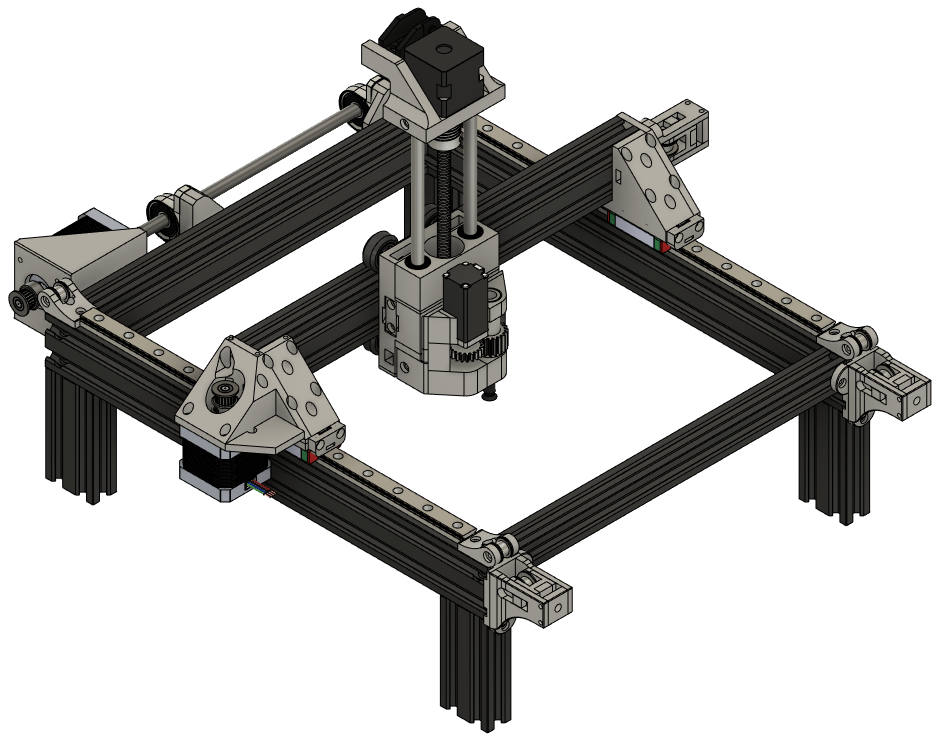
\includegraphics[width=0.9\linewidth]{figures/202108/final-assembly.png}
	\caption{Final robotic subsystem assembly.}
	\label{fig:final-assembly}
\end{figure}

\pendsign

\section[2021/08/24]{Tuesday, 24 August 2021}

\subsection{Component Manufacturing}

I have a personal 3D printer available and therefore it was decided to manufacture the custom components designed for the robotic subsystem using this 3D printer. One of the most commonly used filaments for 3D printing is \ac{PLA} primarily due to the fact that it is easier to print. However, \ac{PLA} has a low glass transition temperature of $50^{\circ}C$. This means that it is possible for the plastic to soften if left in direct sunlight. For this and other reasons, PLA is usually used for art prints as opposed to engineering prints. A filament more suited to engineering applications is \ac{PETG}. \ac{PETG} has a higher glass transition temperature of $80^{\circ}C$ which is much better suited to everyday conditions. Furthermore, \ac{PETG} has mechanical properties that make it less likely to mechanically fail than \ac{PLA}. Therefore, it was chosen to use \ac{PETG} to manufacture the custom components using \ac{FDM} 3D printing techniques. \ac{PETG} has the drawback that it is more challenging to print than \ac{PLA}. In order to achieve successful prints, all of the custom components were printed using a build plate temperature of $85^{\circ}C$ and a nozzle temperature of $240^{\circ}C$. Furthermore, blue painters tape was first placed on the glass build plate to improve build plate adhesion along with rafts. However, the rafts needed to be manually cut away after the print had completed while the blue painter's tape had to be softened by soaking in IPA alcohol before being removed. \FigRef{fig:3d-printed-components} shows all of the custom components printed using the method described over the course of approximately one week. The majority of the components were printed using 0.12 mm layer height to best capture the intricate part details.

\begin{figure}[H]
	\centering
	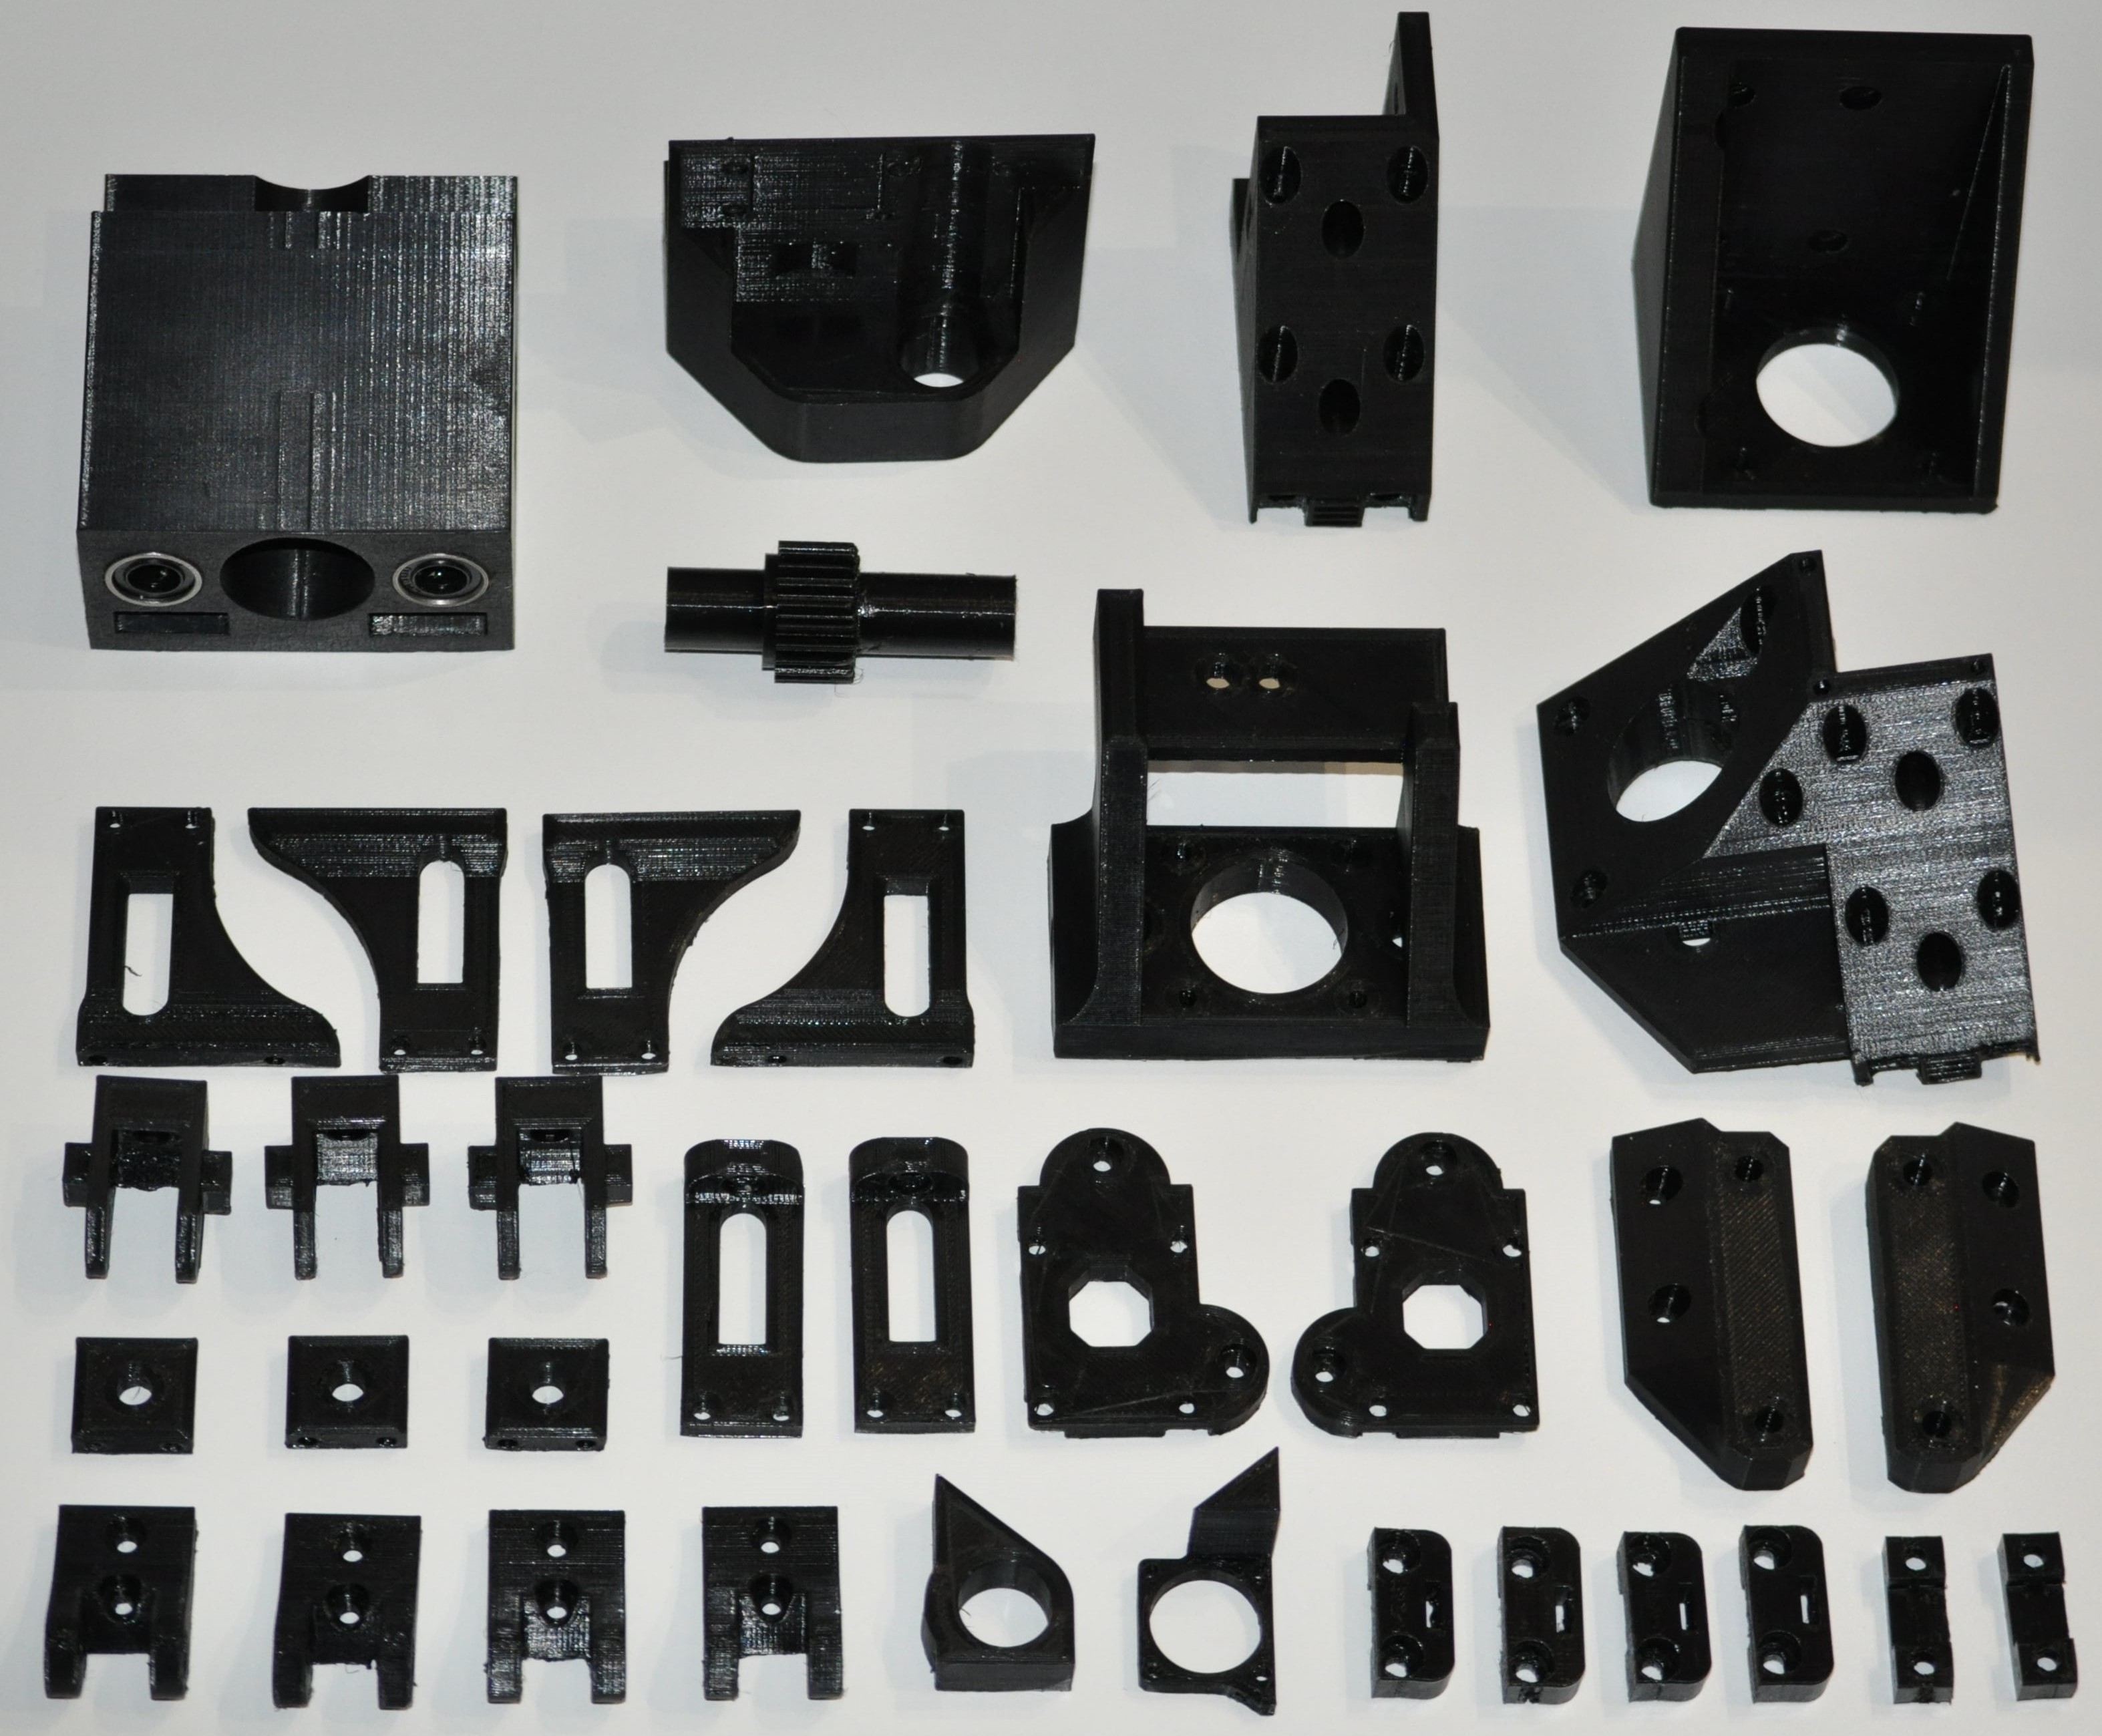
\includegraphics[width=0.7\linewidth]{figures/202108/3d-printed-components.JPG}
	\caption{All the robotic components that were manufactured by means of \ac{FDM} 3D printing methods.}
	\label{fig:3d-printed-components}
\end{figure}

\pendsign

\section[2021/08/27]{Friday, 27 August 2021}

\subsection{Metal Component Machining}

 A number of metal components including aluminium v-slot extrusions, chromed steel linear rods, linear rails and a stainless steel leadscrew were required in order to construct the robotic subsystem. These components could only be purchased in set lengths and therefore needed to be cut to the correct length for the project. Since the length of components such as the y-axis rail spacer extrusions and the leg extrusions affected the accuracy of the robotic subsystem (in terms of consistency of height and distance between the linear rails), the components needed very close to their design length. Therefore, a tolerance of 0.1 mm for the component lengths was specified. Furthermore, in order to facilitate the joining of aluminium extrusions in the design, M5 threads of 20mm depth needed to be tapped into the ends of some of the aluminium extrusions. M5 clearance holes also needed to be drilled through the extrusions along with the corresponding counterbores. Again the tolerance specified for this was 0.1 mm. The high accuracy required for these tasks required specialised machinery. In order to acquire access to such machinery, I approached the Heavy Machinery Lab at the University of Pretoria and was able to acquire access to use the machinery.

The following list summarises the structural components as procured as well as the lengths each of the original components needed to be cut into:

\begin{compactitem}
	\item 1m 2040 aluminium v-slot extrusion: Cut into 3 x 80mm and 2 x 370mm lengths
	\item 1m 2040 aluminium v-slot extrusion: Cut into 1 x 80mm, 1 x 280mm and 1 x 320mm lengths
	\item 1m 2020 aluminium v-slot extrusion: Cut into 2 x 250mm and 1 x 370mm lengths
	\item 1m 2020 aluminium v-slot extrusion: Cut to length 280mm
	\item 1m 8mm diameter chromed steel rod: Cut into 2 x 195mm and 1 x 213mm lengths
	\item 1m, 12mm x 8mm, stainless steel linear rail: Cut into 2 x 320mm lengths
	\item 300mm 8mm diameter stainless steel lead screw: Cut to length 168mm
\end{compactitem}

\begin{figure}[H]
	\centering
	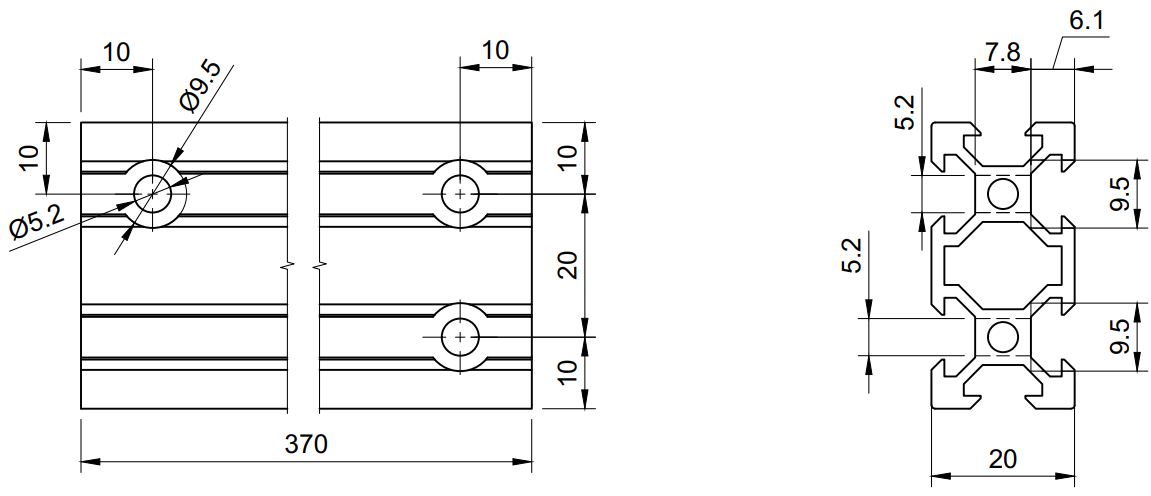
\includegraphics[width=0.7\linewidth]{figures/202108/hg2-001-drawing.png}
	\caption{Technical drawing showing the M5 clearance holes to be cut into the left y-axis 2040 aluminium v-slot extrusion.}
	\label{fig:hg2-001-drawing}
\end{figure}

In order to cut the components to the correct length, a bandsaw to cut the component with approximately 1 mm excess. The bandsaw does not produce a perfectly straight or square cut and the tolerance is relatively high. In order to attain the 0.1 mm tolerance specification, the milling machine was used to shave the excess material of the face of the component to an accuracy of approximately 10 microns. \FigRef{fig:hg2-001-drawing} and \FigRef{fig:hg2-002-drawing} show the technical drawings for the M5 clearance holes that needed to be cut into the y-axis extrusions to facilitate joining of the components to the frame. The drawings were created to be sent in for review during the application process to access the Heavy Machinery Lab. Across the course of three days in the Heavy Machinery Lab, all the required tasks were completed barring the length milling of 6 of the extrusions. It is estimated this will take another day to complete subject to the demand of the milling machine. \FigRef{fig:machined-components} shows the current state of the machined components.

\begin{figure}[H]
	\centering
	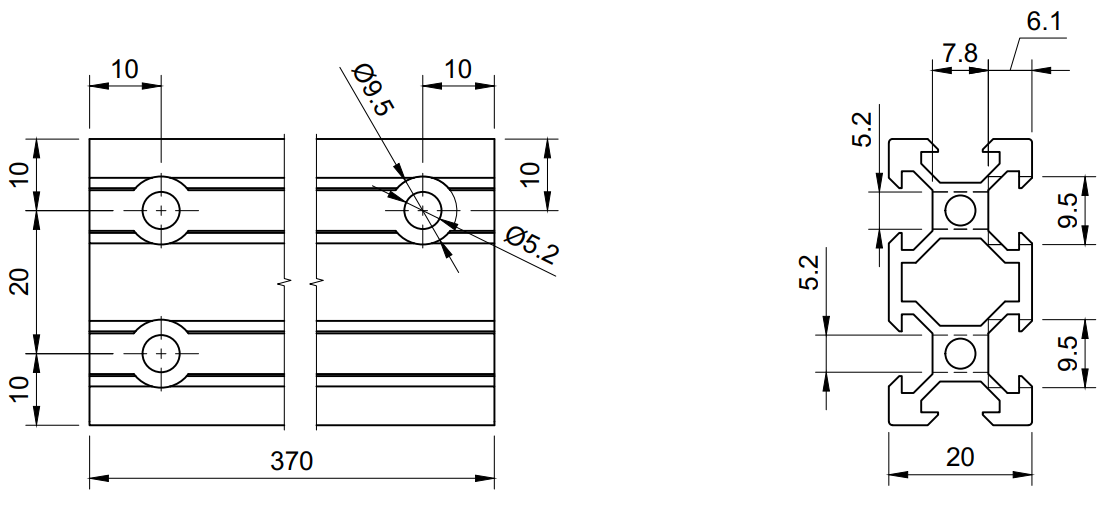
\includegraphics[width=0.7\linewidth]{figures/202108/hg2-002-drawing.png}
	\caption{Technical drawing showing the M5 clearance holes to be cut into the right y-axis 2040 aluminium v-slot extrusion.}
	\label{fig:hg2-002-drawing}
\end{figure}

\begin{figure}[H]
	\centering
	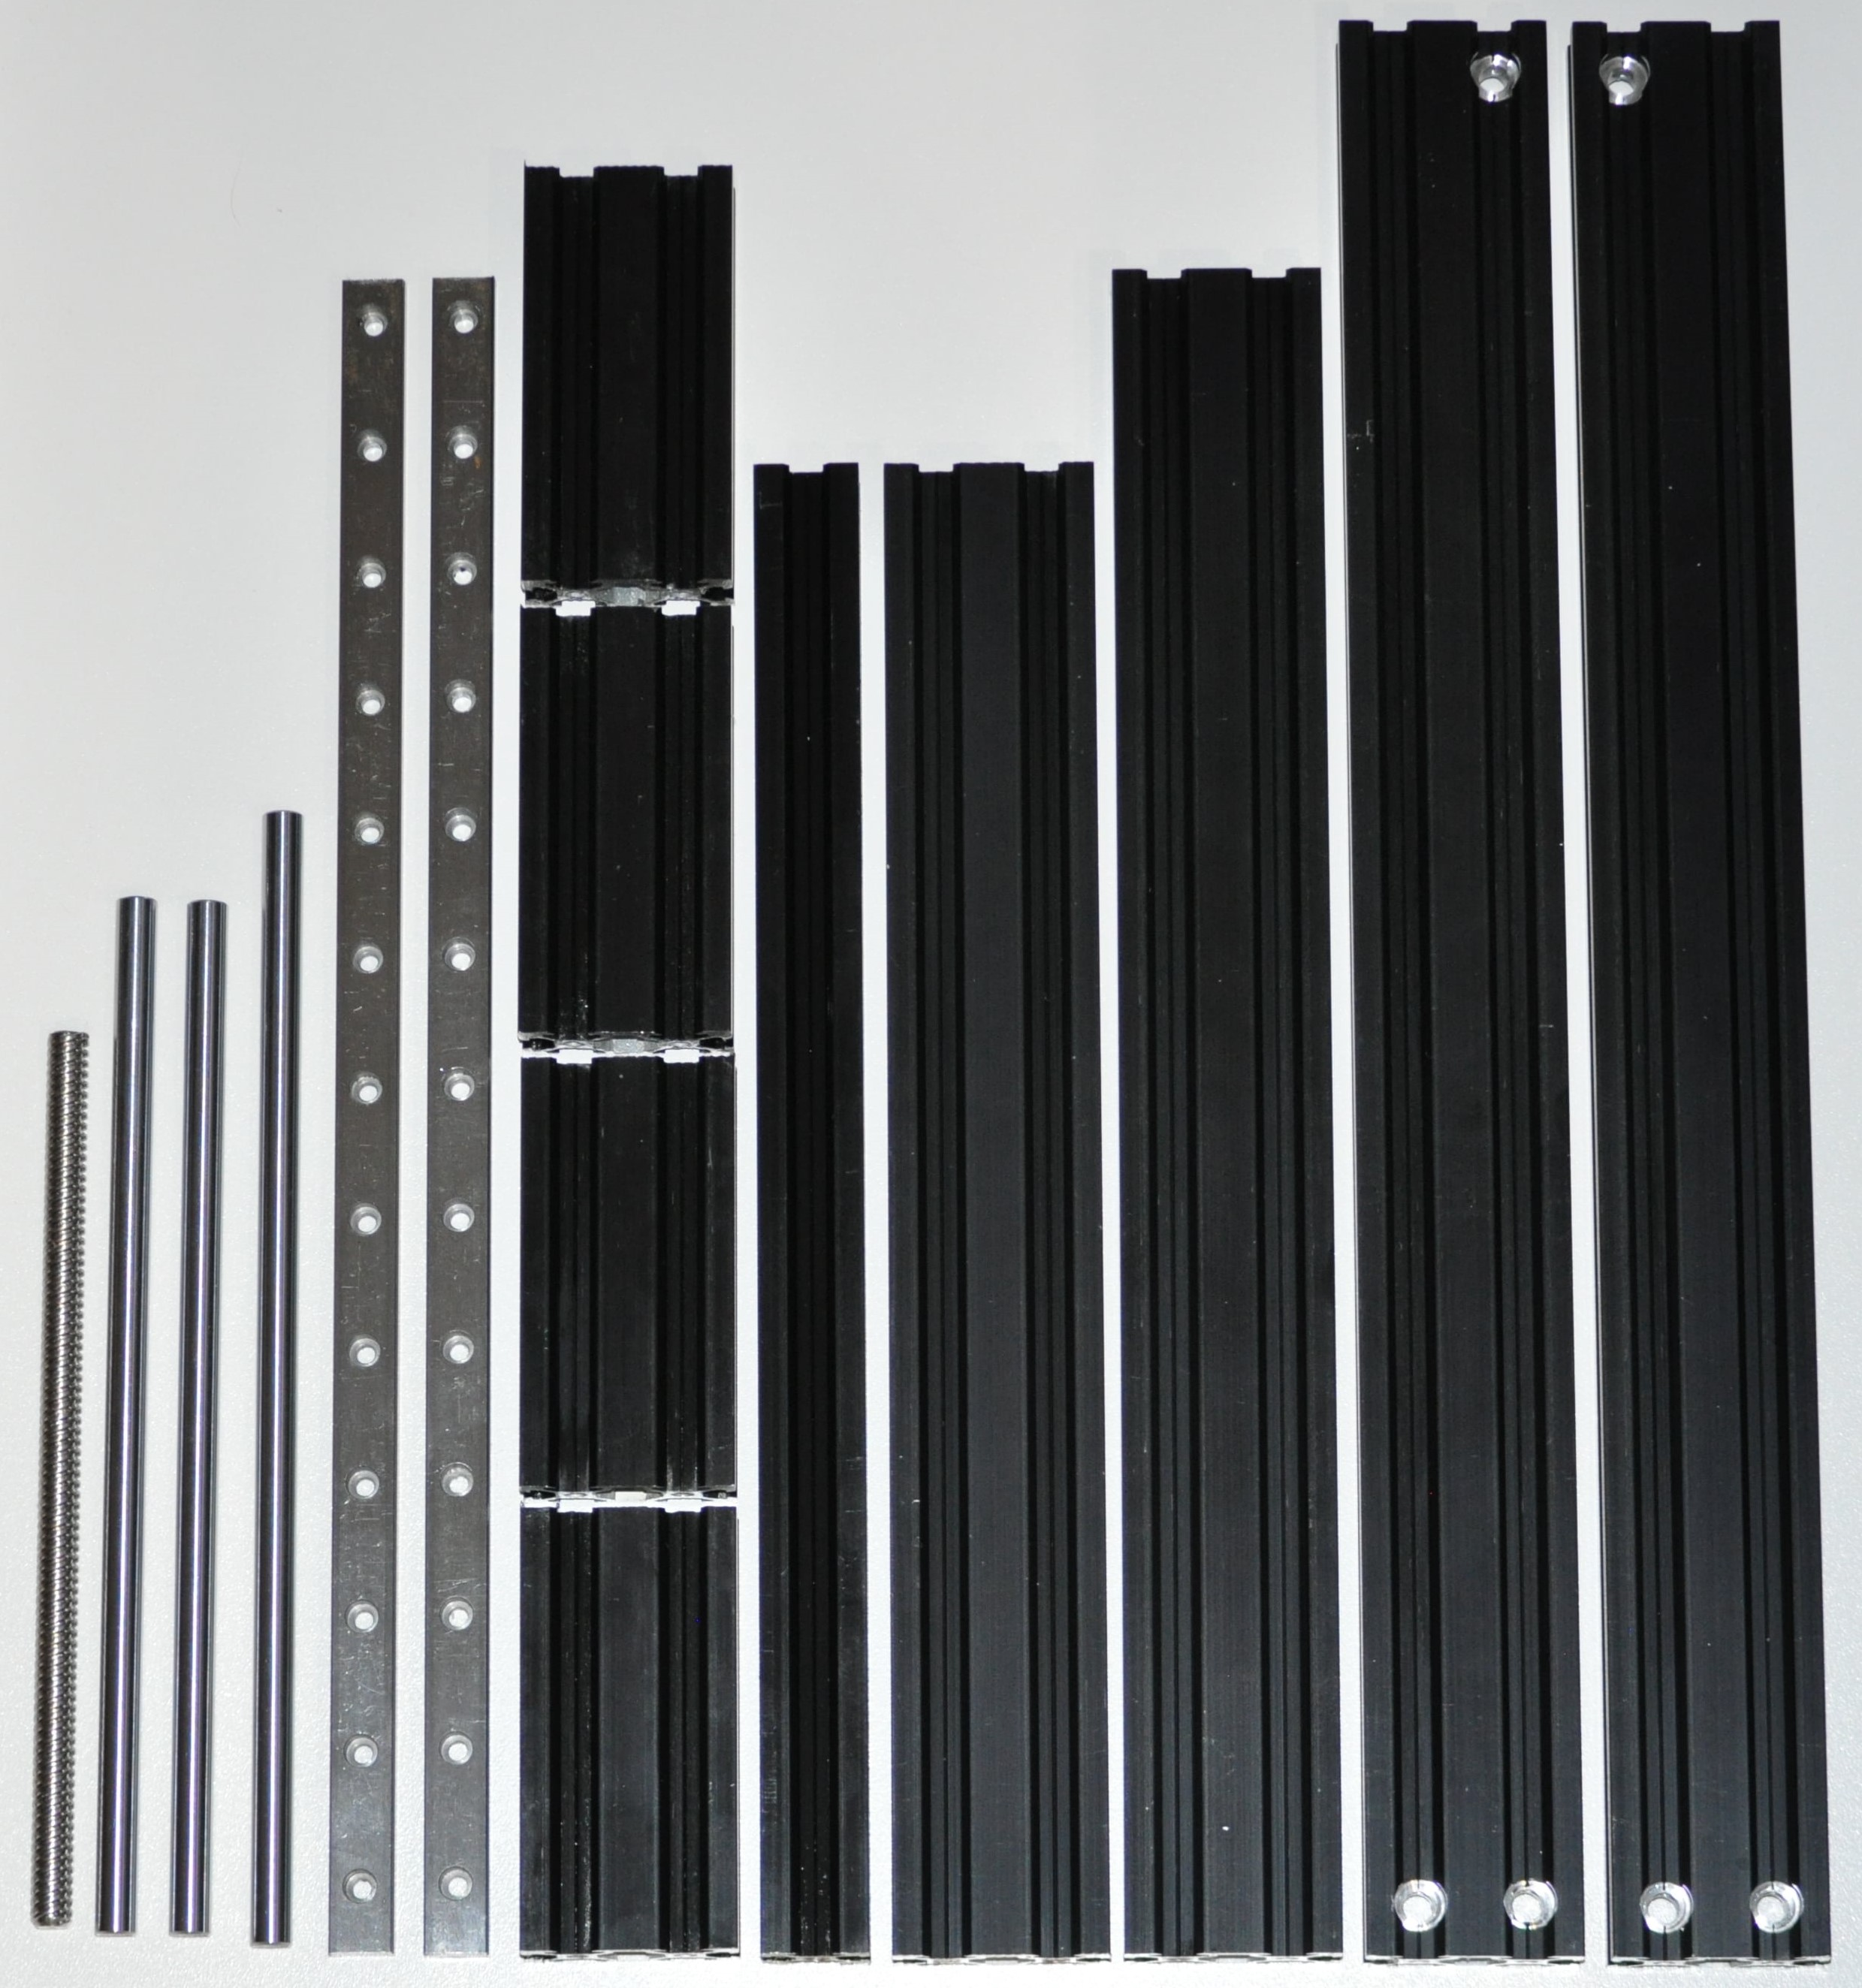
\includegraphics[width=0.5\linewidth]{figures/202108/machined-components.JPG}
	\caption{Metal components after the machining process.}
	\label{fig:machined-components}
\end{figure}

\pendsign

\section[2021/08/28]{Saturday, 28 August 2021}

\subsection{PC-Based Software}

\subsubsection{Initialisation}

Visual Studio 2019 is used as the development environment for creating the PC-based \ac{GUI} software. As discussed previously, the QT C++ framework is used as the basis for the software. In order to facilitate the use of this framework in Visual Studio, the \textit{QT Visual Studio Tools} extension was installed. This was done by accessing the \textit{Extensions > Manage Extensions} menu in Visual Studio. In order to create the Visual Studio project in which the software would be developed, a new project of type \textit{QT Widgets Application} was created. The base class for the project was selected as \textit{QWidget} in the QT Widgets Application wizard that executed when the project was created. When building the project for the first time, a number of errors were generated. This was due to the fact that Visual Studio selected the C++ 14 standard by default for the project when the QT libraries make use of C++ 17 conventions. In order to remedy this issue, the C++ standard for the project was updated from C++ 14 to C++ 17. This was done so by changing the C++ language standard setting located at \textit{Project > Properties > C/C++ > Language > C++ Language Standard} in Visual Studio to \textit{ISO C++17 Standard (/std:c++17)}. The project was successfully compiled and the application executed after updating this setting.

\subsubsection{Software Requirements}

The core requirements that the PC-based software needs to fulfil are as follows:

\begin{compactitem}
	\item The software needs to capture the desired 3D shape to be constructed from the user.
	\item The software needs to provide a visualisation of the shape to be constructed to the user to verify the captured shape is correct.
	\item The software needs to interface with the camera hardware to receive the image input data from the camera.
	\item The software needs to process the image data to detect and localise the cubes input image data.
	\item The software needs to display the raw and annotated camera image data to the user to show the image processing functionality to the user.
	\item The software needs to the utilise the 3D shape input information in conjunction with the processed image information to generate instructions for the robot to construct the 3D shape.
	\item The software needs to convert the robot instructions into a format corresponding to the serial communication protocol between the robot and the computer before sending this data to the robot.
	\item The software needs to monitor the status of the robotic subsystem based on data received from the robot.
	\item The software needs to support the initialisation of the necessary system qualification tests.
	
\end{compactitem}

\pendsign

\section[2021/08/29]{Sunday, 29 August 2021}

\subsection{Robotic Subsystem Construction}

With the custom components manufactured using 3D printing, the supporting components acquired and the metal components mostly machined, the construction of the robotic subsystem could finally begin. Note since the linear rails still needed to be machined to length and cleaned, it was only possible to construct the robot to the completion of the y-axis assembly. Once the final machining is complete, the robotic subsystem can be fully constructed. The construction process primarily consisted of connecting custom, procured and machined components using M3 and M5 machine screws. The combination of these components required to construct the x-axis assembly are shown in \FigRef{fig:physical-x-axis-assembly} with \FigRef{fig:disassembled-x-axis-assembly} showing the components before assembly and \FigRef{fig:assembled-x-axis-assembly} showing the mechanism after assembly. Note the gear on the end-effector motor still needs to be 3D printed. Furthermore, the vacuum rod experienced an issue during printing which prevented the insertion of the vacuum components. Therefore, this part will also have to be re-printed to rectify the issue.

\begin{figure}[H]
	\centering
	\begin{subfigure}[b]{0.7\textwidth}
		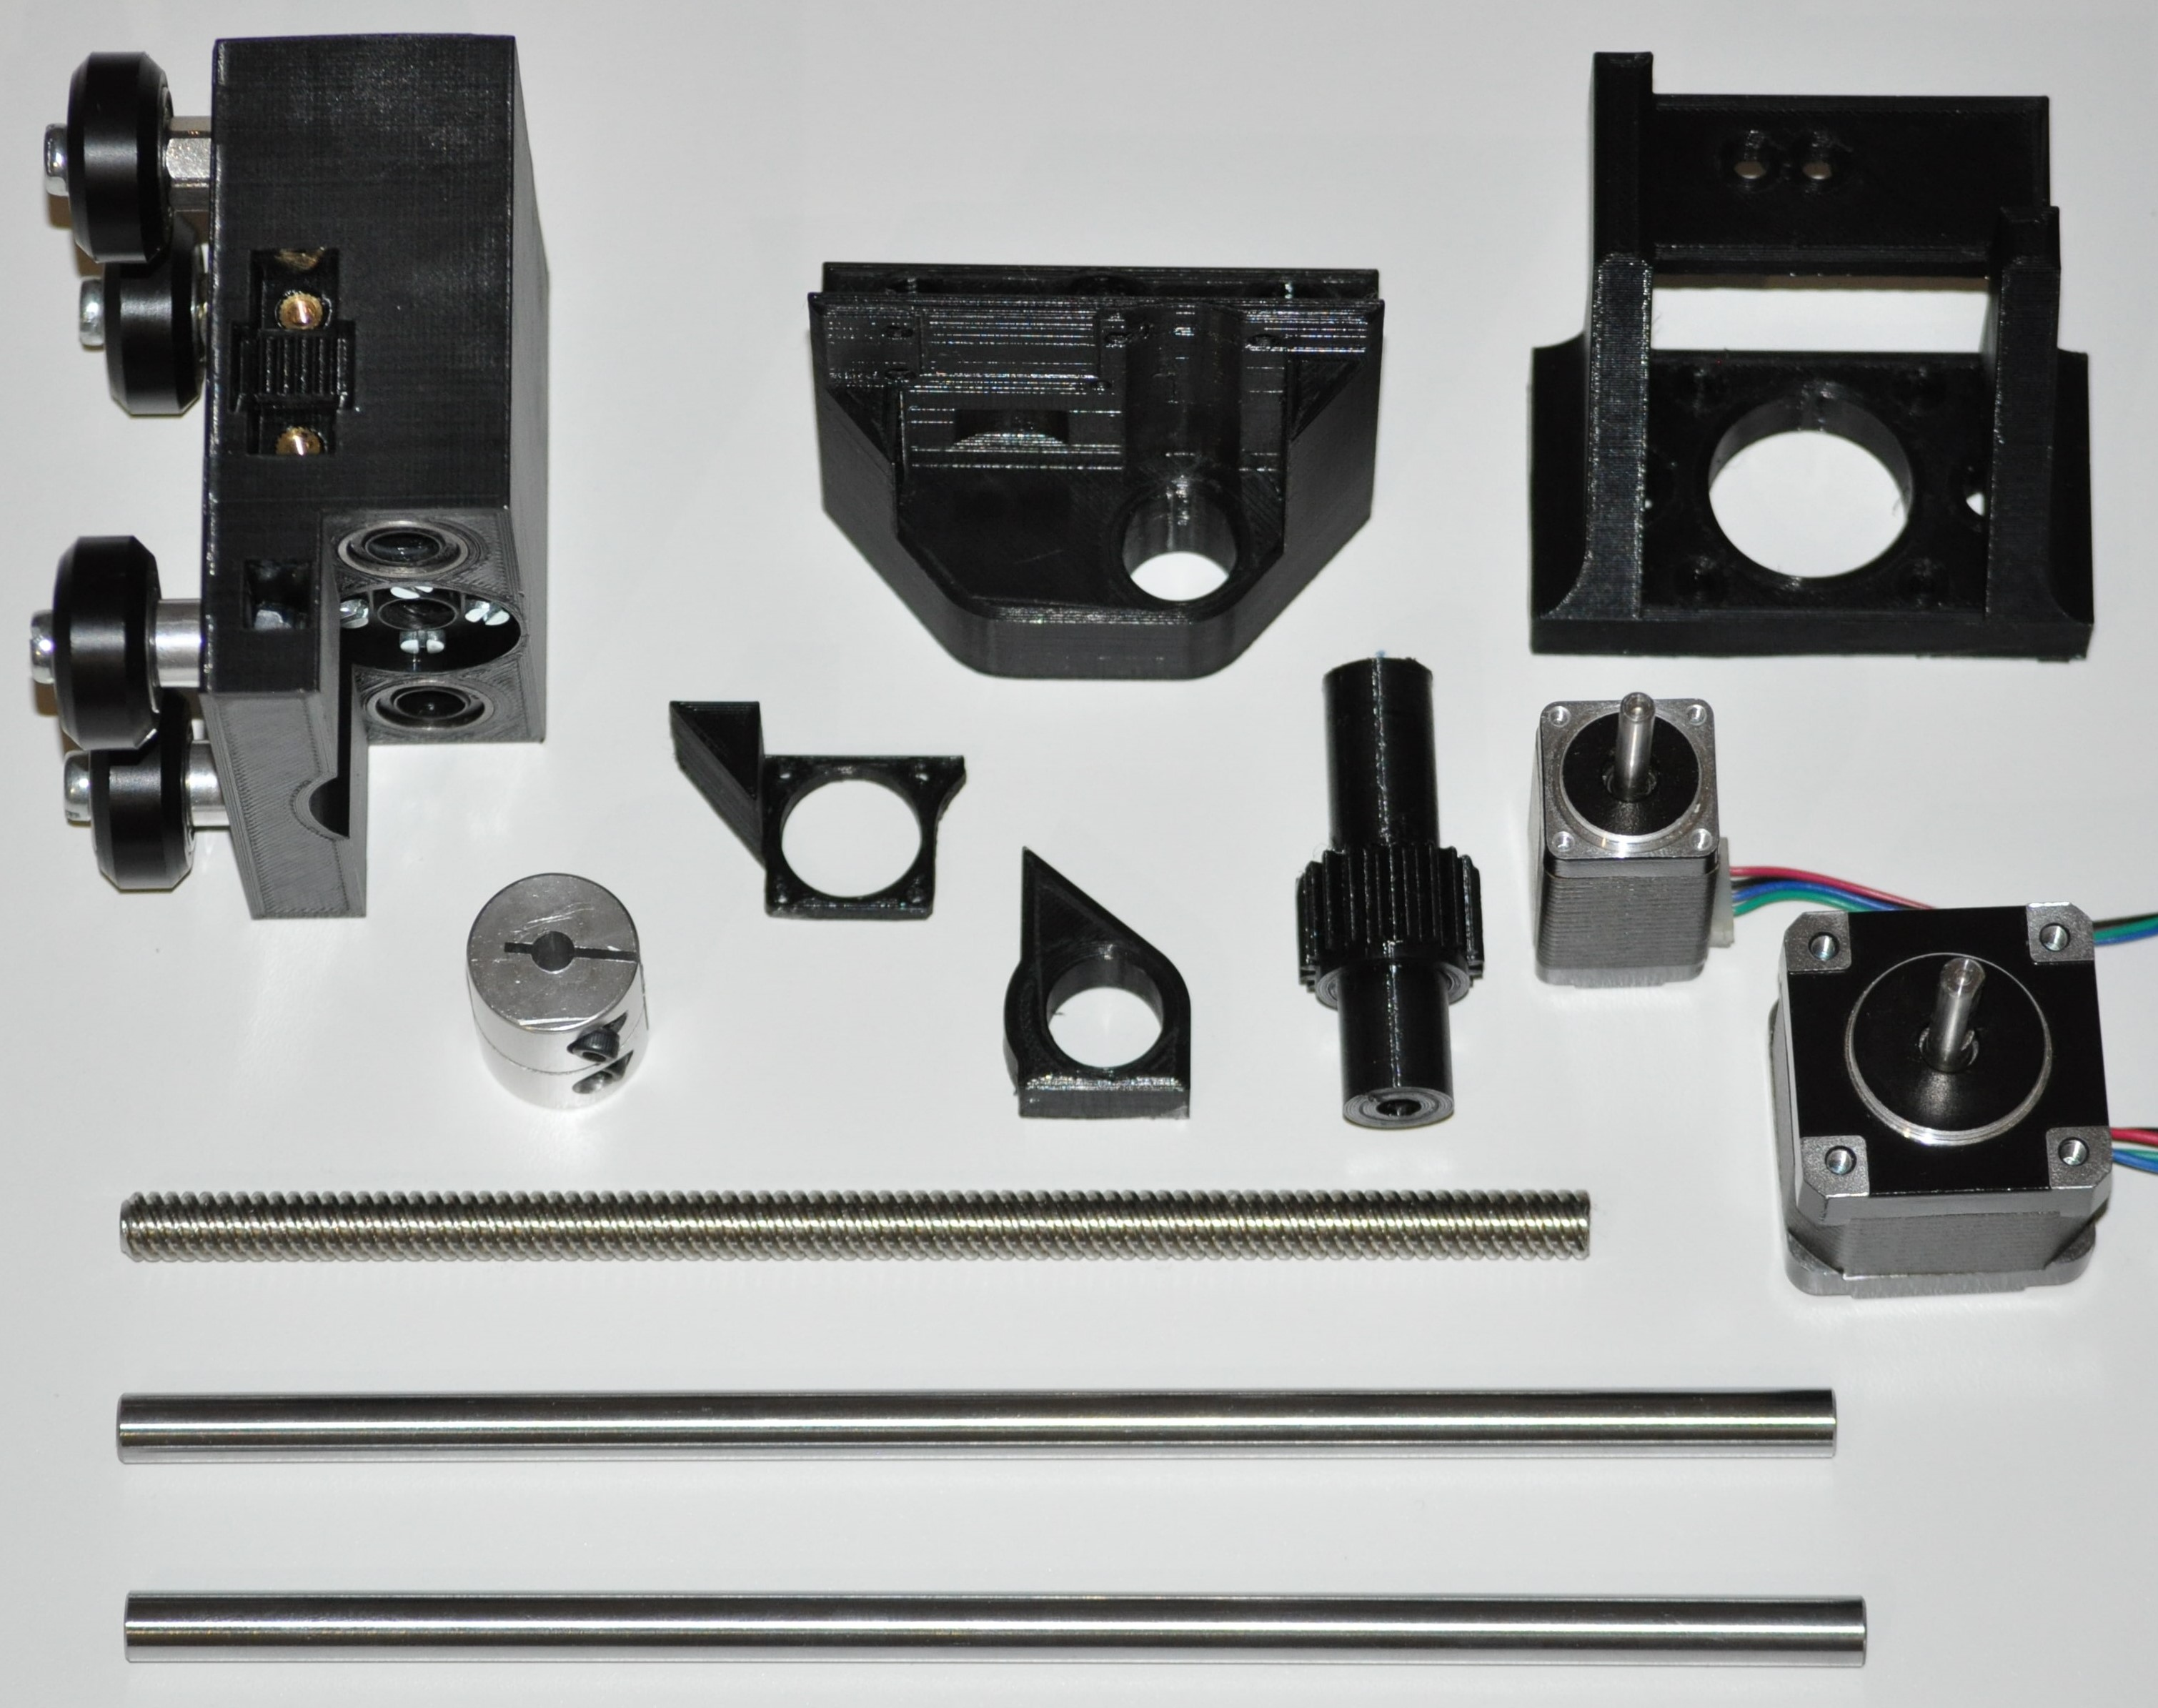
\includegraphics[width=\textwidth]{figures/202108/disassembled-x-axis-assembly.JPG}
		\caption{Components required to construct the x-axis assembly.}
		\label{fig:disassembled-x-axis-assembly}
	\end{subfigure}
	\begin{subfigure}[b]{0.212\textwidth}
		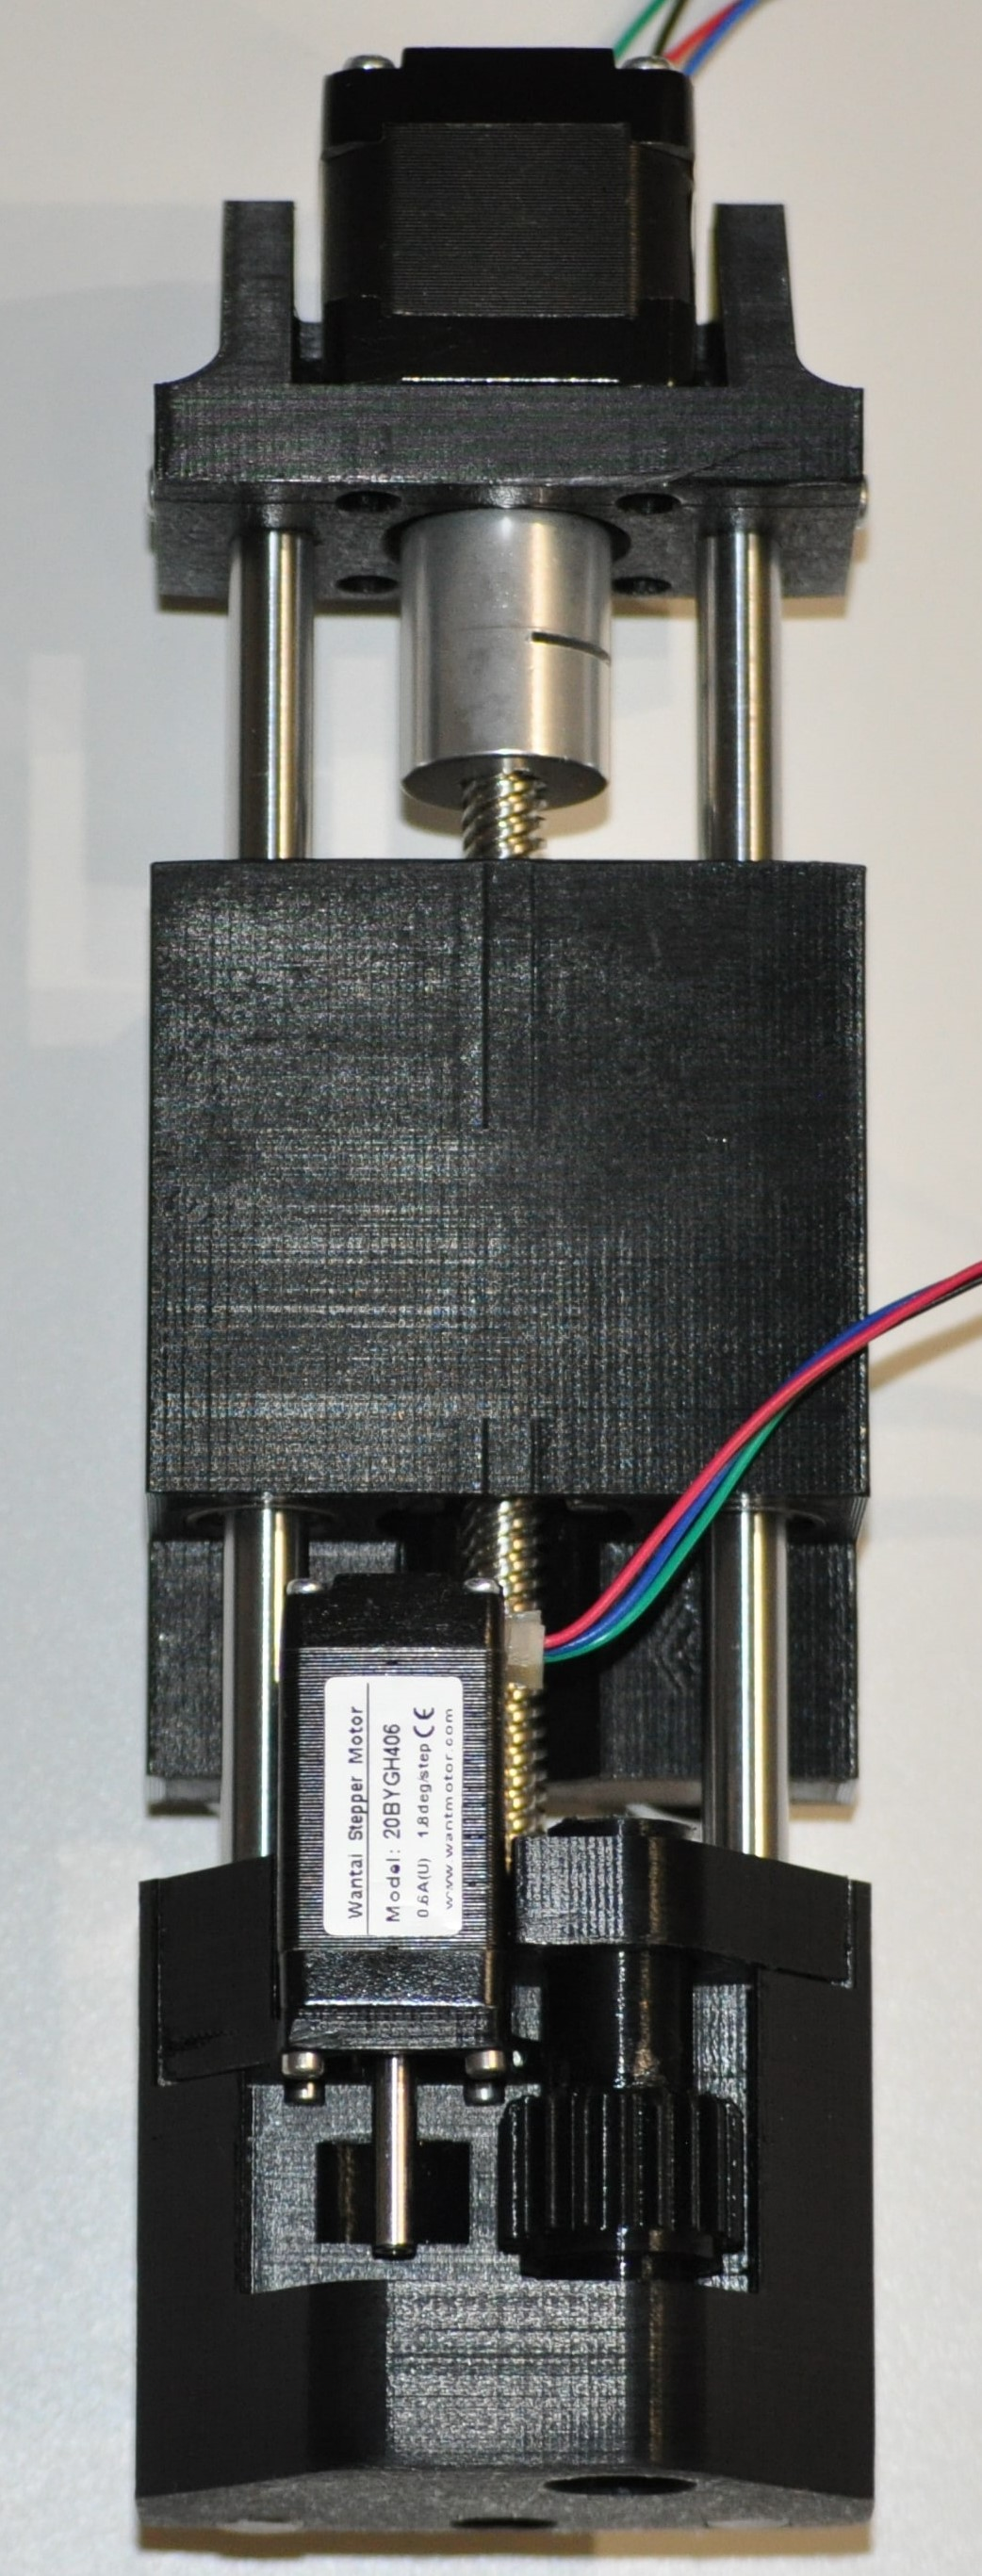
\includegraphics[width=\textwidth]{figures/202108/assembled-x-axis-assembly.JPG}
		\caption{X-axis assembly.}
		\label{fig:assembled-x-axis-assembly}
	\end{subfigure}
	\captionsetup{singlelinecheck = false, justification=justified}
	\caption{X-axis assembly shown in disassembled as well as assembled state.}
	\label{fig:physical-x-axis-assembly}
\end{figure}

The x-axis assembly is used as one of the components to construct the y-axis assembly. The x-axis assembly along with the other components required to construct the y-axis assembly is shown in \FigRef{fig:disassembled-y-axis-assembly}. \FigRef{fig:assembled-y-axis-assembly} shows the assembled y-axis assembly. Note that the timing belt is also included in the assembly despite not being explicitly shown in the components image. Any nuts and bolts required to construct the assembly are also not explicitly shown in \FigRef{fig:disassembled-y-axis-assembly}.

\begin{figure}[H]
	\centering
	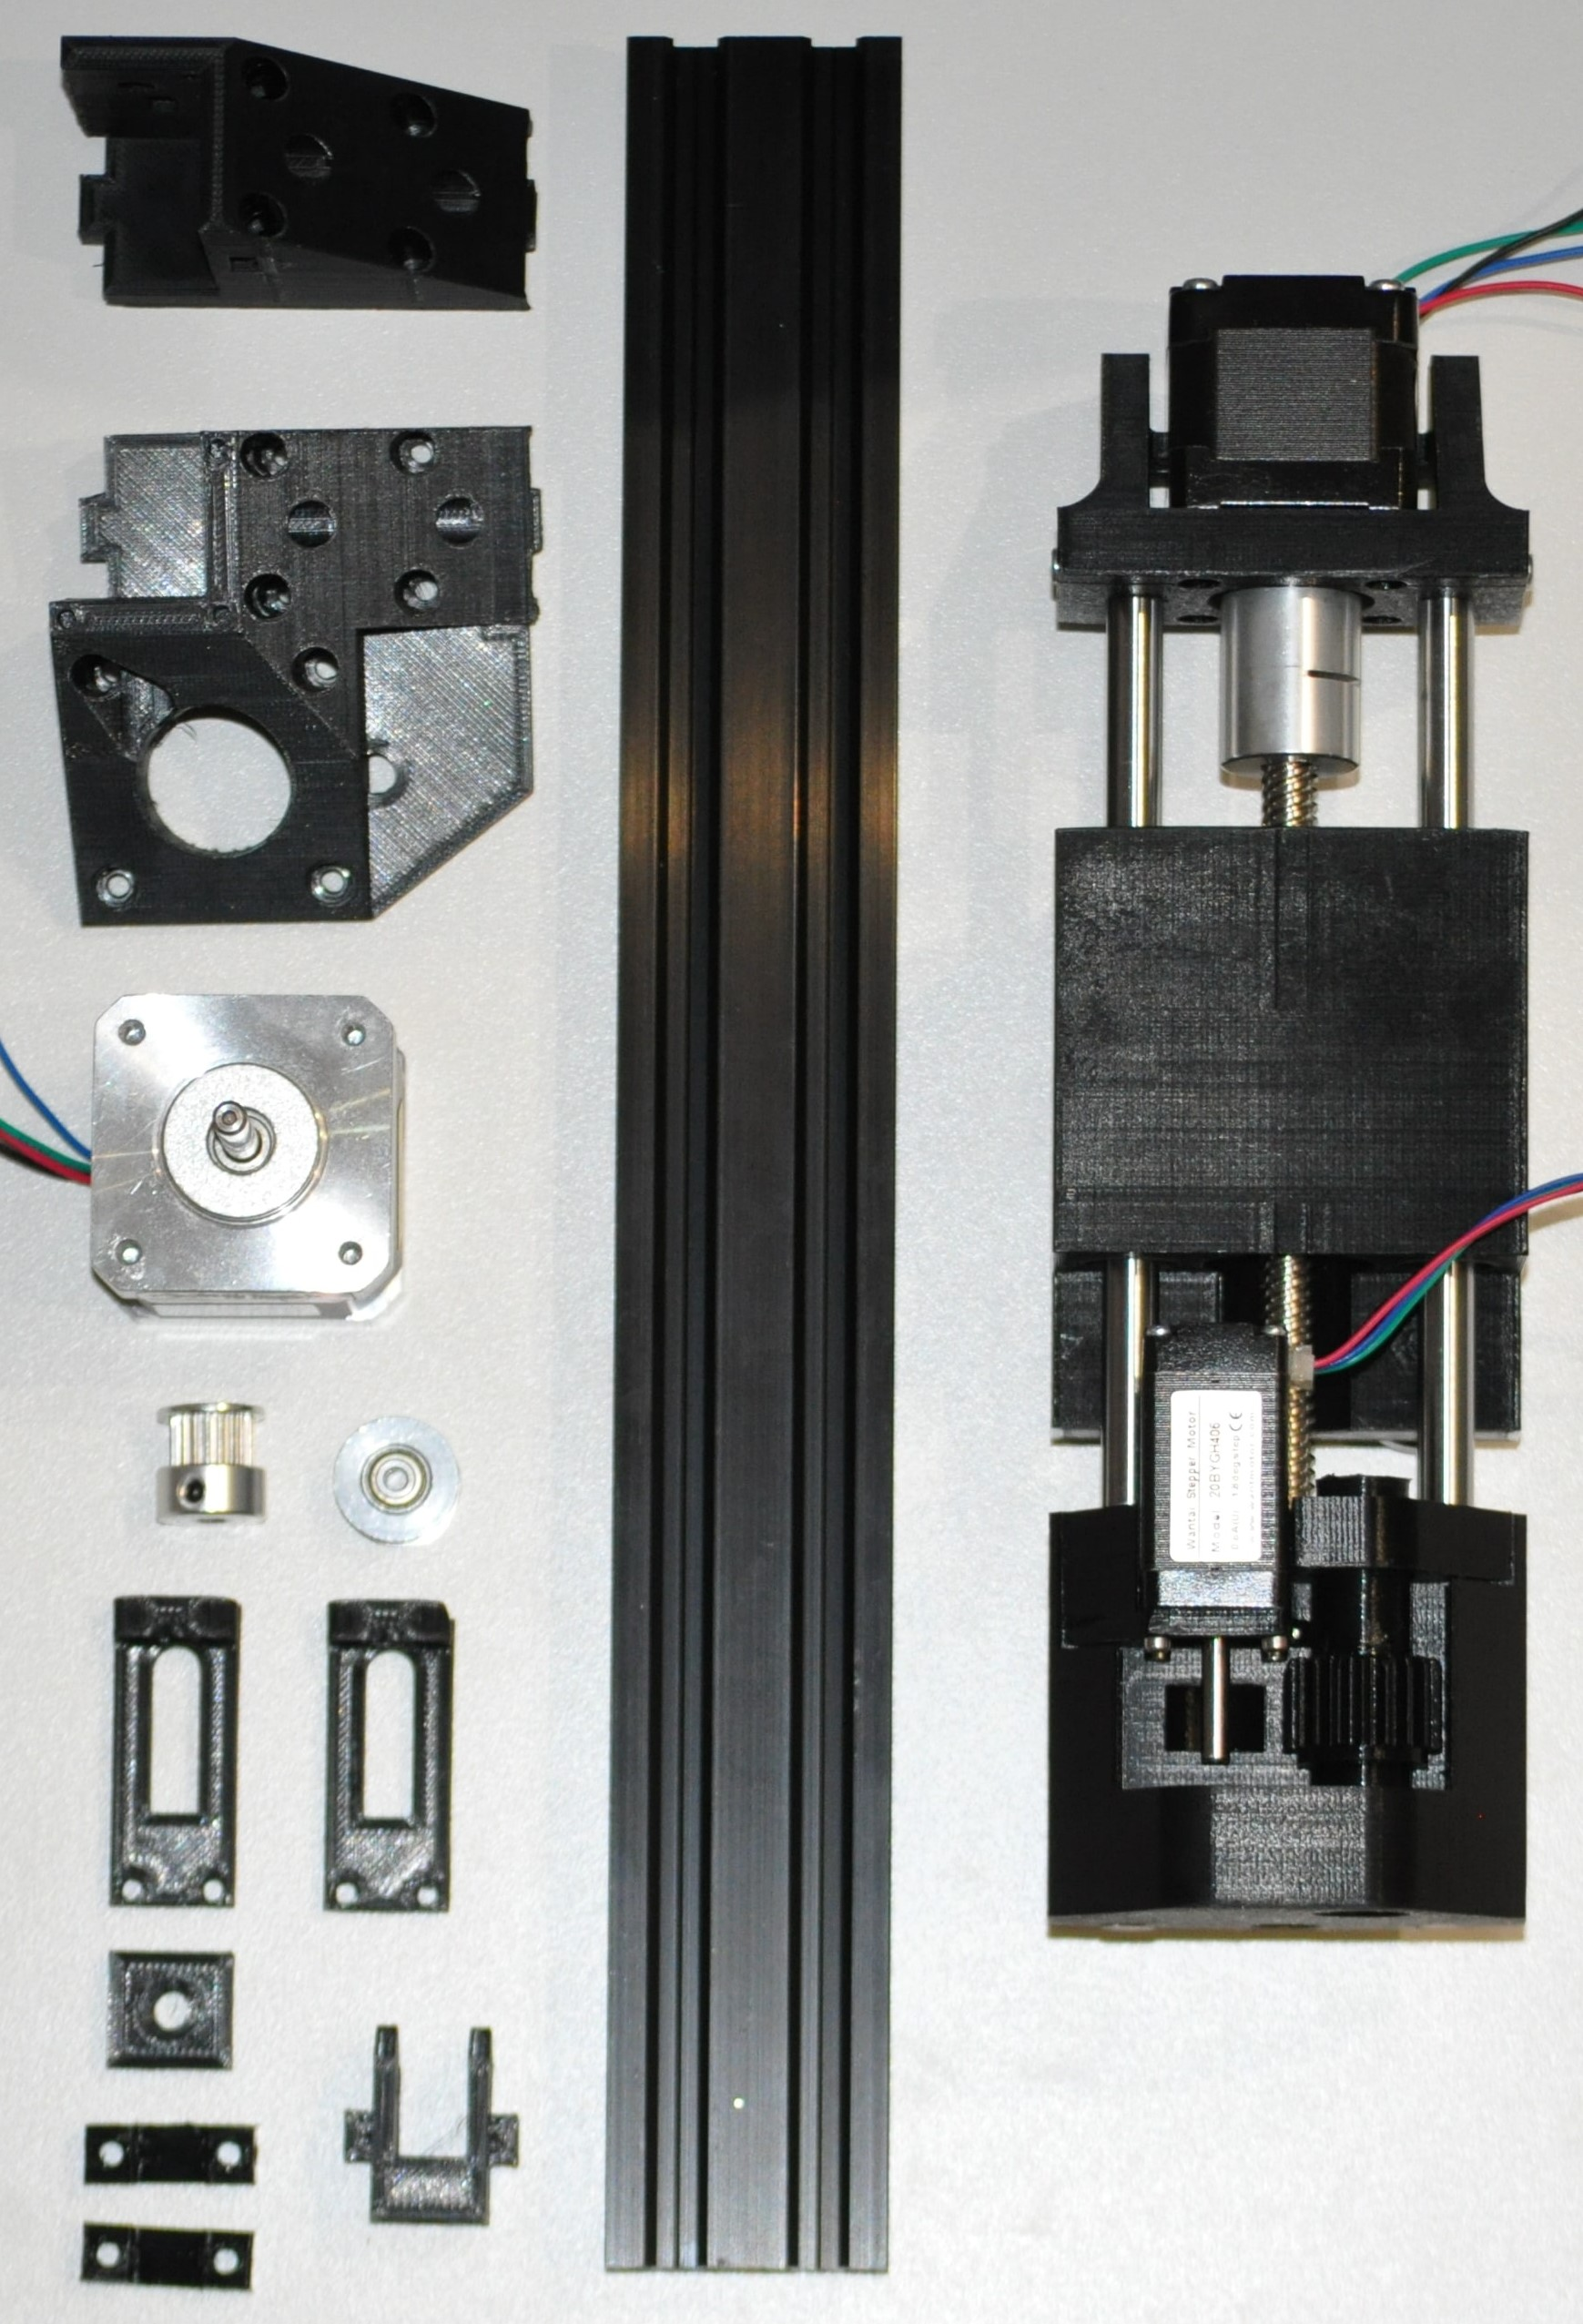
\includegraphics[width=0.4\linewidth]{figures/202108/disassembled-y-axis-assembly.JPG}
	\caption{Components required to construct the y-axis assembly.}
	\label{fig:disassembled-y-axis-assembly}
\end{figure}

\begin{figure}[H]
	\centering
	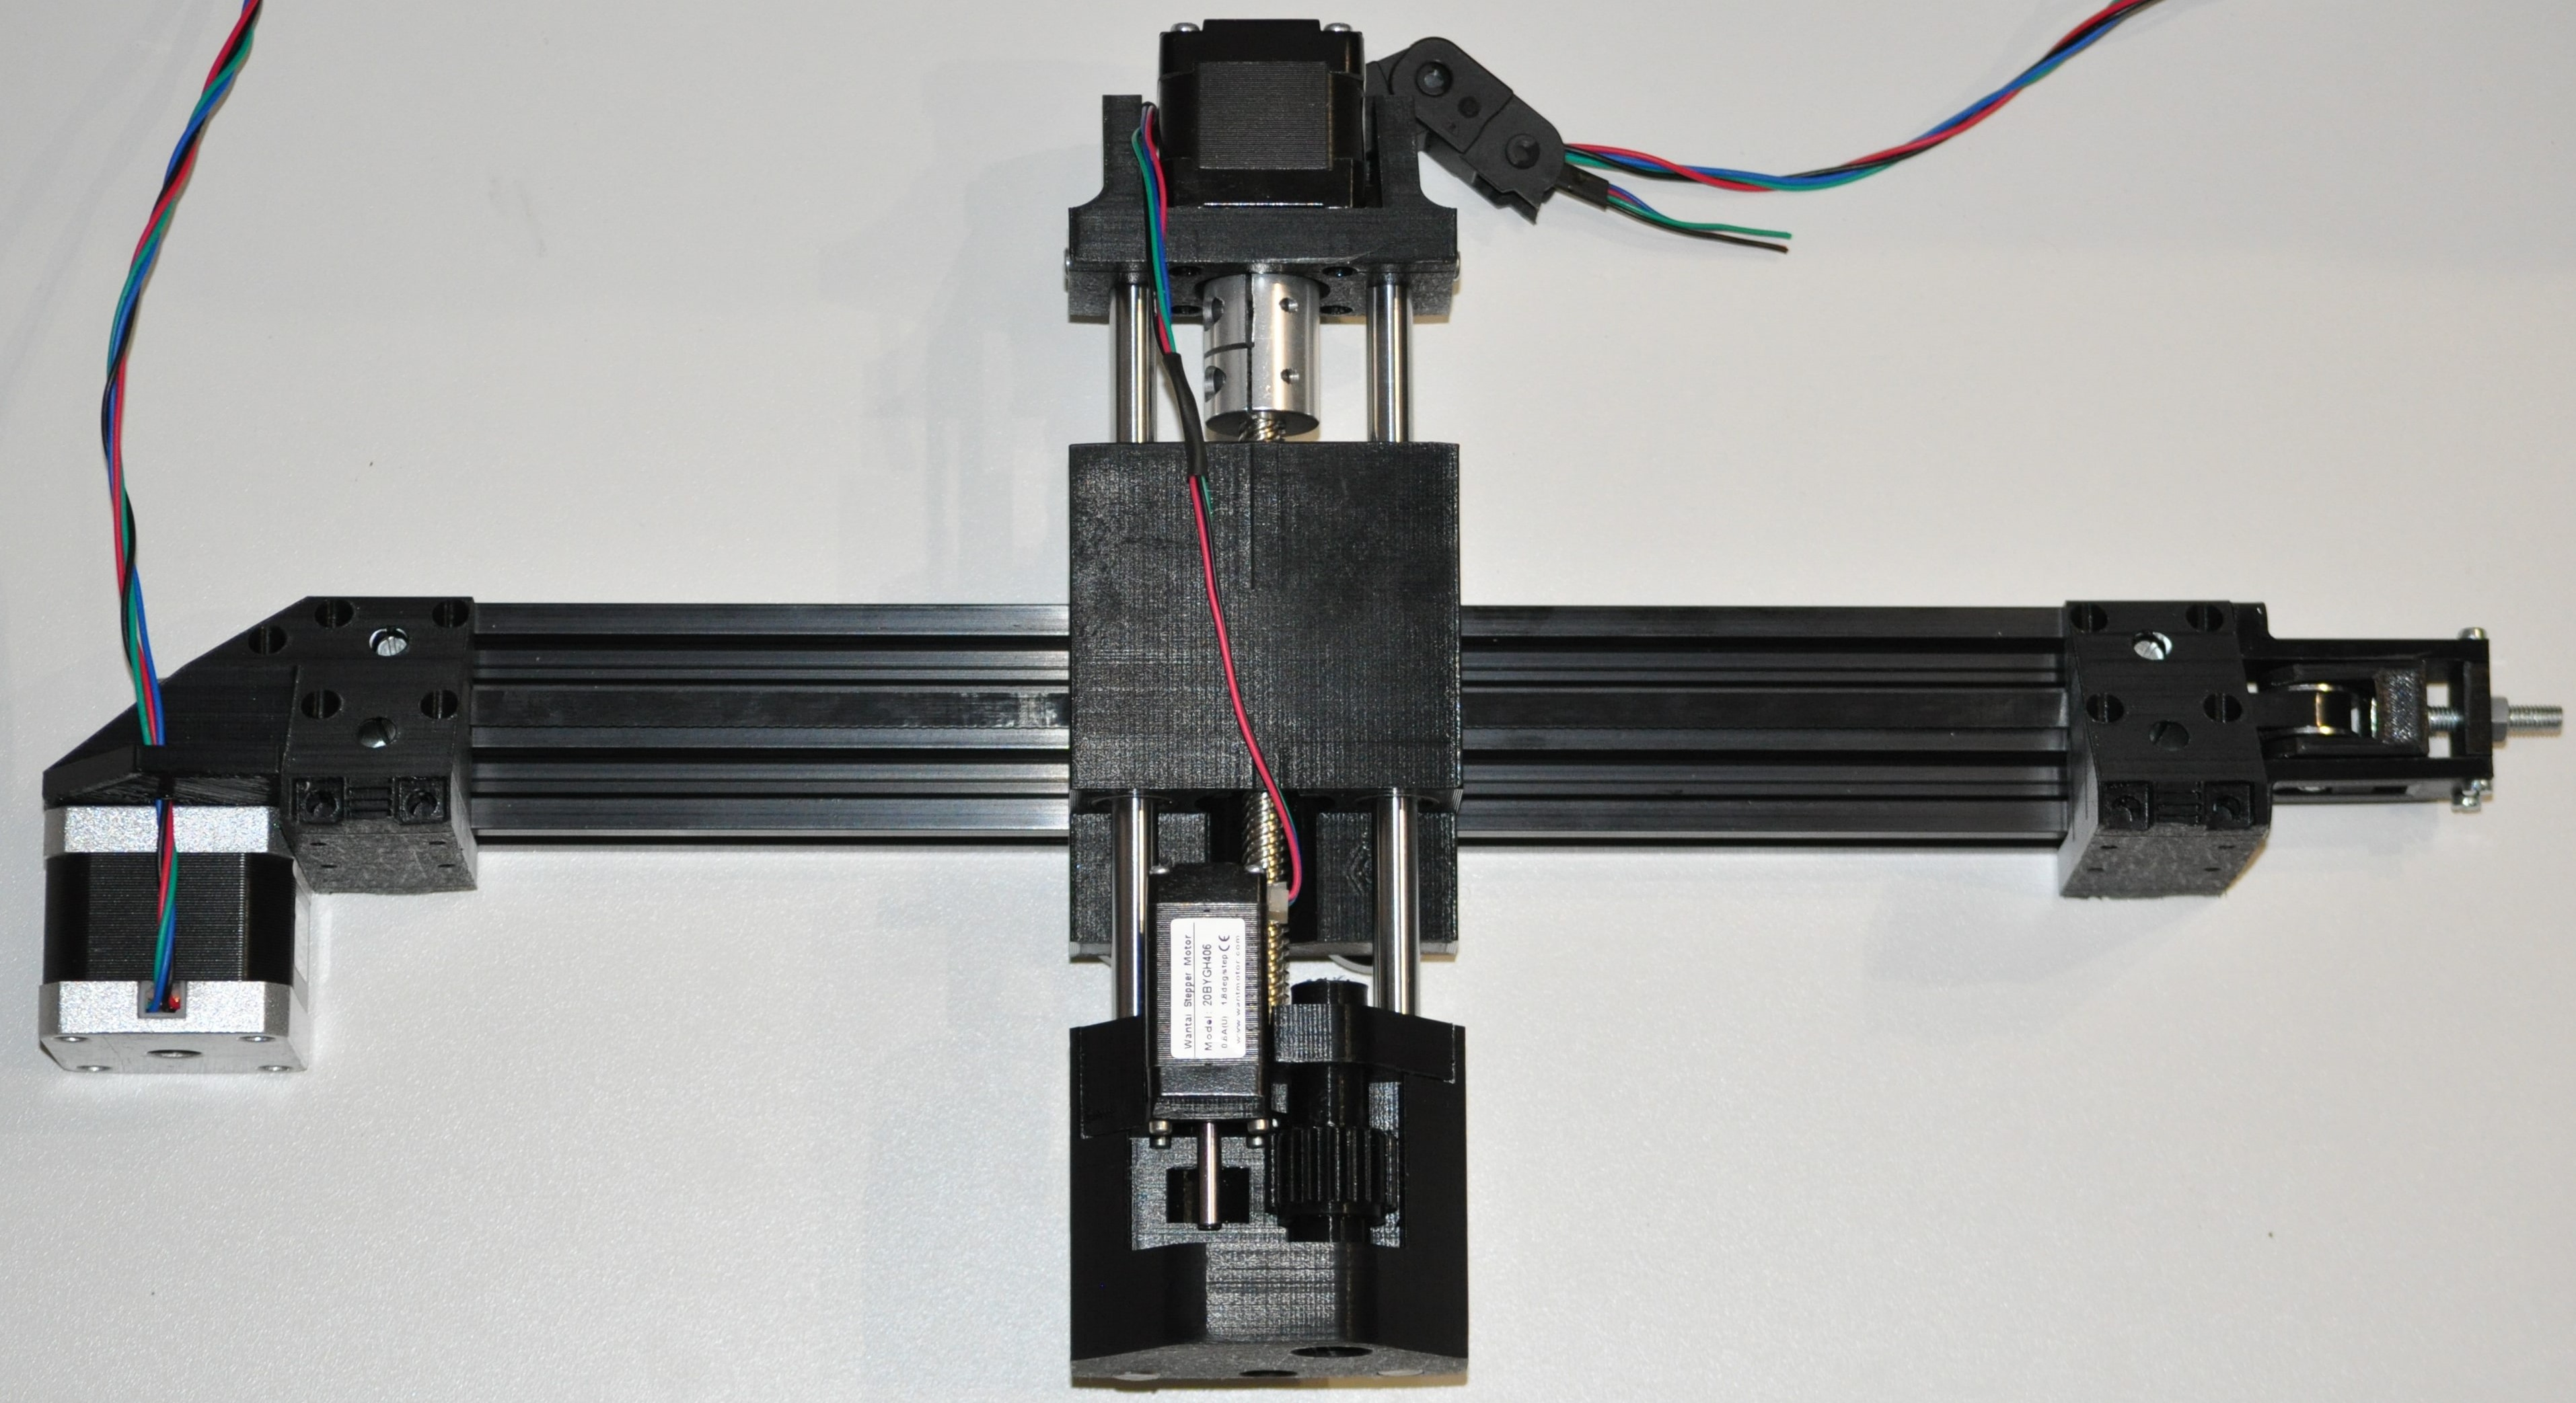
\includegraphics[width=0.8\linewidth]{figures/202108/assembled-y-axis-assembly.JPG}
	\caption{Assembled y-axis assembly.}
	\label{fig:assembled-y-axis-assembly}
\end{figure}

\pendsign